%document
\documentclass[10pt]{beamer}
%theme
\usetheme{metropolis}
% packages
\usepackage{color}
\usepackage{listings}
\usepackage[ngerman]{babel}
\usepackage[utf8]{inputenc}
\usepackage{multicol}

\usepackage{hyperref}
\hypersetup{colorlinks=true, linkcolor=blue, urlcolor=red}

% color definitions
\definecolor{mygreen}{rgb}{0,0.6,0}
\definecolor{mygray}{rgb}{0.5,0.5,0.5}
\definecolor{mymauve}{rgb}{0.58,0,0.82}

\lstset{
    backgroundcolor=\color{white},
    % choose the background color;
    % you must add \usepackage{color} or \usepackage{xcolor}
    basicstyle=\footnotesize\ttfamily,
    % the size of the fonts that are used for the code
    breakatwhitespace=false,
    % sets if automatic breaks should only happen at whitespace
    breaklines=true,                 % sets automatic line breaking
    captionpos=b,                    % sets the caption-position to bottom
    commentstyle=\color{mygreen},    % comment style
    % deletekeywords={...},
    % if you want to delete keywords from the given language
    extendedchars=true,
    % lets you use non-ASCII characters;
    % for 8-bits encodings only, does not work with UTF-8
    frame=single,                    % adds a frame around the code
    keepspaces=true,
    % keeps spaces in text,
    % useful for keeping indentation of code
    % (possibly needs columns=flexible)
    keywordstyle=\color{blue},       % keyword style
    % morekeywords={*,...},
    % if you want to add more keywords to the set
    numbers=left,
    % where to put the line-numbers; possible values are (none, left, right)
    numbersep=5pt,
    % how far the line-numbers are from the code
    numberstyle=\tiny\color{mygray},
    % the style that is used for the line-numbers
    rulecolor=\color{black},
    % if not set, the frame-color may be changed on line-breaks
    % within not-black text (e.g. comments (green here))
    stepnumber=1,
    % the step between two line-numbers.
    % If it's 1, each line will be numbered
    stringstyle=\color{mymauve},     % string literal style
    tabsize=4,                       % sets default tabsize to 4 spaces
    % show the filename of files included with \lstinputlisting;
    % also try caption instead of title
    language = C,
	showspaces = false,
	showtabs = false,
	showstringspaces = false,
	escapechar = ,
}

\def\ContinueLineNumber{\lstset{firstnumber=last}}
\def\StartLineAt#1{\lstset{firstnumber=#1}}
\let\numberLineAt\StartLineAt



\newcommand{\codeline}[1]{
	\alert{\texttt{#1}}
}

% This Document contains the information about this course.

% Authors of the slides
\author{
    Lecturers:
	%name1
	Mirko Jantschke,
	%name2
	Pascal Scholz
	\\
	%creaters of the slides
	Created by: Richard Mörbitz, Manuel Thieme
}


% Fancy Logo
\titlegraphic{\hfill
\includegraphics[height=1.25cm]{../templates/fsr_logo_cropped}}


\title{C-Lessons}
\subtitle{Variables}
\date{\today}

\begin{document}

\begin{frame}
	\titlepage
\end{frame}
\begin{frame}{Overview}
	\setbeamertemplate{section in toc}[sections numbered]
	\tableofcontents
\end{frame}

%----------------------------------------------------------------------------------------------------
\section{Motivation}

%----------------------------------------------------------------------------------------------------
\begin{frame}
	\centerline{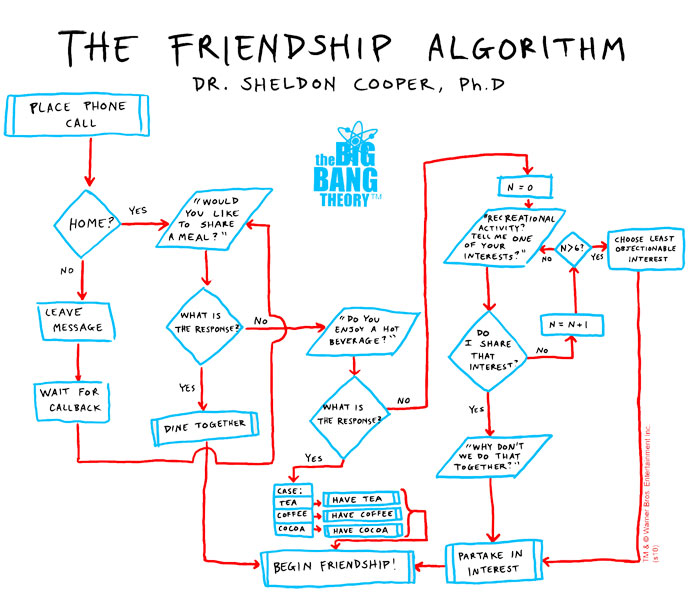
\includegraphics[scale=.32]{../img/friendship.jpg}}
	\bigskip
	Take a look at the right part. It is executed up to seven times.
\end{frame}
%----------------------------------------------------------------------------------------------------
\section{Loops}

%----------------------------------------------------------------------------------------------------
\begin{frame}[fragile]{Loops}
	To repeat statements as long as a certain condition is met, C offers 3 different loops.
	\begin{lstlisting}[numbers=none,basicstyle=\itshape\footnotesize]
while (condition)
    statement;
    \end{lstlisting}
	\begin{lstlisting}[numbers=none,basicstyle=\itshape\footnotesize]
do
    statement;
while (condition);
    \end{lstlisting}
	\begin{lstlisting}[numbers=none,basicstyle=\itshape\footnotesize]
for (initialization; condition; statement)
    statement;
    \end{lstlisting}
	For multiple statements again, use braces.
\end{frame}

%----------------------------------------------------------------------------------------------------
\begin{frame}[fragile]{while}
	The execution of a loop is a continuous alternation between checking if the condition is still met and executing the statement(s).
	\begin{lstlisting}
int i = 2;
while (i > 0)
	- -i;
printf("done\n");
\end{lstlisting}
	\begin{enumerate}[<+(1)->]
		\item Check (i $>$ 0) $\rightarrow$ \textbf{true} $\rightarrow$ go to line 3
		\item Decrement i $\rightarrow$ i now is \textbf{1}, go back to line 2
		\item Check (i $>$ 0) $\rightarrow$ \textbf{true} $\rightarrow$ go to line 3
		\item Decrement i $\rightarrow$ i now is \textbf{0}, go back to line 2
		\item Check (i $>$ 0) $\rightarrow$ \textbf{false} $\rightarrow$ go to line 4
		\item Print \textbf{done}
	\end{enumerate}
\end{frame}

%----------------------------------------------------------------------------------------------------
\begin{frame}[fragile]{do...while}
	The difference between \textit{do...while} and \textit{while} is the order of executing the statement(s) and checking the condition.\\
	\bigskip
	The \textit{while} loop begins with checking, while the \textit{do...while} loop begins with executing the statement(s).
	\begin{lstlisting}[numbers=none]
int i = 3;
do
	- -i;
while (i < 1);
\end{lstlisting}
	\bigskip
	The Statement(s) in a \textit{do ... while} loop are executed at least once.
\end{frame}

%----------------------------------------------------------------------------------------------------
\begin{frame}[fragile]{for}
	The For-Loop is comfortable for iterating. It takes three arguments.
	\begin{itemize}
		\item Initialization
		\item Condition
		\item Iteration statement
	\end{itemize}
	\bigskip
	For illustration, consider a program printing the numbers 1 to 10:
	\begin{lstlisting}[numbers=none]
int i;
for (i = 1; i <= 10; ++i)
	printf("%d\n", i);
\end{lstlisting}
	\begin{itemize}
		\item \textit{i} is called an \textit{index} iterating from the given start to a given end value
		\item \textit{i, j, k} are commonly used identifiers for the index
	\end{itemize}
\end{frame}

%----------------------------------------------------------------------------------------------------
\section{Miscellaneous}
\begin{frame}[fragile]{Meanwhile...}
	Be careful, this
	\begin{lstlisting}[numbers=none]
while (1 > 0)
	printf("Did you miss me?\n");
\end{lstlisting}
runs till the end of all days.\\
\ \\$\infty$ loops are common mistakes, and you will experience many of them.\\
Check for conditions that are always true.
\end{frame}

%----------------------------------------------------------------------------------------------------
\begin{frame}[fragile]{for ever}
	The arguments for the \textit{for loop} are optional. E.g. if you already have defined your iterating variable:
	\begin{lstlisting}[numbers=none]
int i = 1;
for (; i <= 10; ++i)
	printf("%d\n", i);
\end{lstlisting}
	Or if you have the iteration statement in your loop body:
	\begin{lstlisting}[numbers=none]
for (i = 1; i <= 10;)
	printf("%d\n", ++i);   /* seems more like a while loop */
\end{lstlisting}
	And if you're not passing anything, it runs \textbf{for}ever:
	\begin{lstlisting}[numbers=none]
for (;;)
	printf("I'm still here\n");
\end{lstlisting}
Note: the semicolons are still there.
\end{frame}

%----------------------------------------------------------------------------------------------------
\begin{frame}{Cancelling loops}
	\textit{break}
	\begin{itemize}
		\item Ends loop execution
		\item Moves forward to first statement after loop
	\end{itemize}\ \\\ \\
	\textit{continue}
	\begin{itemize}
		\item Ends current loop iteration
		\item Moves forward to next step of loop iteration
		\begin{itemize}
			\item\textit{while:} Jumps to condition
			\item\textit{for:} Jumps to iteration statement
		\end{itemize}
	\end{itemize}
\end{frame}

%----------------------------------------------------------------------------------------------------
\begin{frame}[fragile]{Saving code lines}
	You can define variables inside the initialization part of a for loop.
	\begin{lstlisting}[numbers=none]
for (int i = 1; i <= 10; ++i)
	printf("%d\n", i);
\end{lstlisting}
	\ \\\ \\In that case, the variable is only available inside the for loop (as if it was declared in the body).\\
	\begin{lstlisting}
int guess = 0;
int solution = 42;
for (int i = 1; guess != solution; ++i)
	scanf("%d", &guess);
printf("Tries: %d\n", i);   /* invalid! */
\end{lstlisting}
	This feature was added in the C99 standard.
\end{frame}

%----------------------------------------------------------------------------------------------------
\begin{frame}[fragile]{Compiler options}
	When calling \textit{gcc}, you can pass several options to it:\\
	\bigskip
	\begin{tabular}{|l|l|}
		\hline
		\textbf{option} & \textbf{description} \\\hline
		-std=c99 & Use C99 as the standard \\\hline
		-o $<$name$>$ & output file is \textit{name} instead of \textit{a.out} \\\hline
		-Wall & Enable all compiler warnings \\\hline
		-Wextra & Enable even more compiler warnings \\\hline
		-Werror & Treat warnings as errors \\\hline
	\end{tabular}\\
	\bigskip
	Example:
	\begin{lstlisting}[numbers=none]
$ gcc -std=c99 -o main main.c
\end{lstlisting}
\end{frame}

%----------------------------------------------------------------------------------------------------
\begin{frame}[fragile]{A few words on style}
	\begin{itemize}
        \item Stay consistent after deciding whether to use or not to use braces on a single statement
		\item If you skip the loop body
		\begin{itemize}
			\item Leave a comment in your code
			\item Use an extra line for the empty statement
		\end{itemize}
	\end{itemize}
		\begin{lstlisting}[numbers=none]
for (i = 1; i < 9; printf("%d\n", ++i));    /* confusing */

for (i = 1; i < 9; printf("%d\n", ++i))     /* clear */
    ;/* do nothing */
\end{lstlisting}
\end{frame}

%----------------------------------------------------------------------------------------------------

\end{document}
